\renewcommand{\chaptername}{\scshape Partie}
\chapter{\normalfont \scshape Dispositif à onde de choc}
\section{Théorie du tube à choc}
\section{Protocole et organisation}
\subsection{Cahier des charges}
Après avoir déterminé les objectifs relatifs au dispositif à onde de choc, le diagramme de GANTT suivant a été établi :
\begin{figure}[H]
	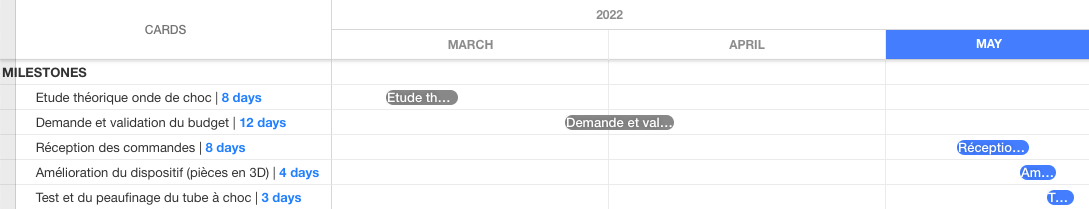
\includegraphics[scale = 0.4]{figures/gantt_choc.png}
	\caption{\small{\textit{Diagramme de GANTT prévu pour le dispositif à onde de choc}}}
	\label{gantt_choc}
\end{figure}
Le travail sur le tube à onde de choc a été confié aux trois membres restants du groupe. Le tableau ~\ref{gestion_choc} résume les postes attribués à chacun des membres:
\begin{table}[H]
	\centering
	\begin{tabular}{|l l l|}
		\hline
		\small\textbf{Responsable onde de choc}&\small\textbf{Responsable sécurité}&\small\textbf{Responsable technique}\\
		\hline
		\small{Nivo VIVIAND}&\small{Hovanes BOKSYAN}&\small{Aymeric FREREJEAN}\\
		\hline
	\end{tabular}
	\caption{\small\textit{Membres et tâches attribuées (tube à onde de choc)}}
	\label{gestion_choc}
\end{table}
\subsection{Mise en place du dispositif}
\section{Observations et conclusion}
\subsection{Description des résultats}
\subsection{Interprétation}
\subsection{Conclusion partielle}